\documentclass{article}

\usepackage[utf8]{inputenc}
\usepackage[french]{babel}
\usepackage{graphicx}

\usepackage{hyperref}
\hypersetup{
    colorlinks=true,
    linkcolor=red,
    filecolor=magenta,
    urlcolor=blue,
}

\urlstyle{same}

\graphicspath{{ressources/}}

\title{UE 3I013: Projet Recherche\\
    Encadrante: Vanda Luengo\\
    SuperViseur: Rapport}

\author{Basile Pesin}

\begin{document}

\maketitle
\newpage

\tableofcontents
\newpage

\section{Rappel des problématiques et hypothèses principales}

\subsection{Groupes de références}
Comme vu dans le document de compréhension, l'objectif de cette étude~\cite{SuperViseur} est de relever les comportements mis en oeuvres par les enseignants en face de leur classe, et plus particulièrement de déterminer les caractéristiques du "groupe de référence", c'est a dire le sous-ensemble d'élèves qui bénéficie du plus d'attention de la part des enseignants, et sur lesquels ceux ci s'appuient pour prendre des décisions. On cherchera entre autres à relever la taille de ce groupe de référence.

\subsection{Différences entre novices et expérimentés}
On tentera aussi de vérifier les différences comportementales (qu'on suppose importantes) entre enseignant novices (2 et 3) et expérimentés (1 et 4). Entre autres on voudra vérifier que les enseignants expérimentés ont moins de difficulté à évaluer l'état de la classe et à y réagir. Pour que les différences entre enseignants soient facilement visibles, il faudra clairement juxtaposer et mettre en parallèle les visualisations concernant les différents enseignants (tout en évitant de surcharger l'utilisateur d'informations).

\subsection{Objectifs de formation}
Puisque ces visualisations mettent en valeur les (on espère bons) comportements d'enseignants expérimentés, ou pourra utiliser les résultats obtenus, au dela de leur intérêt théorique, à des fins de formations. Les visualisations réalisées doivent donc être facilement manipulables et interprétables par des personnes n'étant pas membre de la communauté scientifique. On portera donc un soin particulier à l'ergonomie du site construit.

\section{Choix techniques}
Afin de pouvoir aisément présenter les résultats de l'étude à la communauté scientifique, ainsi qu'a la communauté éducative à des fins pédagogiques, il a été décidé de rendre les visualisations disponibles sous forme d'un site web. Même si cela s'éloigne légèrement du fonctionnement d'\href{https://undertracks.imag.fr}{Undertracks}, ou les opérateurs sont écrits en Python, on pourrait imaginer mettre à l'avenir en place un système similaire à celui \href{http://superviseur.lip6.fr}{superviseur.lip6.fr}, ou des opérateurs Python générent des morceaux de codes HTML/Javascript à "imbriquer" dans le reste du code.\\
Le résultat du travail est visible \href{https://vertmo.github.io/SuperViseur/}{ici}. L'intégralité du code source est également disponible sur \href{https://github.com/Vertmo/SuperViseur}{GitHub}.

\subsection{Bibliothèques JavaScript}
Afin de simplifier le développement, on a utilisé plusieurs bibliothèques de fonctionnalités JavaScript:
\begin{itemize}
    \item \href{https://jquery.com/}{jQuery} qui permet de facilement manipuler le DOM (Document Object Model) HTML. Cette bibliothèque permet également de simplifier les requètes ajax (qui permettent entre autre de charger les données de l'étude). De plus, c'est une dépendance de la bibliothèque suivante.
    \item \href{https://semantic-ui.com/}{Semantic UI} est un framework HTML/CSS, permettant donc de créer un site web d'aspect convenable rapidement.
    \item \href{http://svgjs.com/}{SVG.js} a été choisi pour construire les représentations spatiales et circulaires. Comme son nom l'indique, cette bibliothèque manipule des SVG (Scalable Vector Graphics). (au départ, et comme indiqué dans le document de compréhjsion, on souhaitait utiliser la biblioithèque \href{https://p5js.org/}{p5.js}, mais celle-ci était beaucoup moins pratique pour gérer le survol de souris, et qui plus est elle tendait à créer des fuites de mémoires).
    \item \href{http://www.chartjs.org/}{Chart.js} est une bibliothèque permettant d'afficher des graphiques interactifs. On l'utilise principalement pour résumer les résultats sur la page d'accueil du site.
\end{itemize}

\subsection{Données}
\subsubsection{Tables}
Comme expliqué dans le document de compréhension, les données à traiter pour ce projet se présentent sous la forme de trois fichier csv exportés depuis la plateforme \href{https://undertracks.imag.fr/}{UnderTracks}: \textit{users.csv} qui contient la liste des élèves, \textit{events.csv} qui contient la timeline des évènements, et \textit{context.csv}, qui contient la description des constantes et acronymes utilisés.\\
Ces 3 fichiers sont placés dans le dossier \textit{/data} du projet. On aurait préféré pouvoir charger les données directement depuis la plateforme UnderTracks (via une REST API par exemple) afin de ne pas avoir à stocker les fichiers dans le dépot, mais cela n'est malheureusement pas encore possible.\\
Dans le cadre de ce projet, on utilisera principalement la table des utilisateurs et celle des évènements. On charge ces deux tables en même temps que le site au moyen de requètes Ajax, et on garde les informations chargées en mémoire. Dans le cas des utilisateurs ayant une connexion lente, le chargement de ces tables (en particulier la tables des évènements, qui compte plus de 25000 lignes, ou 6.7Mo de données) peut présenter un léger ralentissement. Heureusement, le fait qu'on ne charge ces données qu'une fois par visite de la page ainsi que le cache du navigateur permettent de réduire le nombre de chargements et donc ce problème.

\subsubsection{Anonymisation des données}
Le projet SuperViseur impliquant la récolte de données sur des élèves de primaire (CP, CE1, CE2) il est très important de correctement anonymiser les données avant de les rendre publiques. Cela signifie, entre autres, que les vidéos enregistrés par le système d'eye tracking ne sont pas accessibles au public, et que les prénoms des élèves ont évidemment été supprimés de la table des utilisateurs avant même la mise en ligne sur UnderTracks. Le problème est que ces prénoms se trouvent aussi dans la verbalisation de l'enseignant (qui s'adresse à ses élèves par leurs prénoms). Même si cela ne permet pas directement d'identifier quel élève porte quel prénom, on peut, en mettant en relation les élèves regardés et ceux nommés par l'enseignant, parvenir à identifier les élèves.\\
On a donc réalisé un petit script (en python) permettant de remplacer les prénoms des élèves par leurs numéros dans la verbalisation de l'enseignant. En plus d'anonymiser les données, cela a l'avantage de permettre de mieux visualiser les relations entre les élèves nommés et les élèves regardés. Bien entendu, ce script contenant lui même une table des correspondances prénoms / numéros des élèves, il n'est pas inclut dans le dépot.

\subsubsection{Position de l'enseignant}
Une information utile dans le cadre de nos visualisations spatiales est la position de l'enseignant dans la classe. En effet, on peut faire l'hypothèse que le regard de l'enseignant se pose plus souvent sur les élèves proches de lui. Le problème est que cette information n'est pas présente dans la transcription des données actuellement disponible (mais elle le sera à l'avenir).\\
Afin de pouvoir malgré tout tester cette fonctionnalité de nos visualisations, on a donc crée une version "factice" de cette donnée, en ajoutant à la table des évènements deux colonnes posX et posY indiquant respetivement la position en X et en Y de l'enseignant (pour les questions de direction des axes, d'origine et d'echelle, on a gardé la convention utilisée pour noter la position des élèves). Dans nos données factices, l'enseignant suit donc une marche aléatoire en deux dimensions: $(posX, posY) \in [0, 40]^2$.

\section{Visualisations}
Pour ce projet, on a réalisé quatre types de visualisations différentes, chacune mettant en valeur certaines informations. Chaque visualisation est présentée sur une des pages du site.
\begin{itemize}
    \item \textbf{Résumé:} La première page visible sur le site présente des résultats globaux sur la distribution des regards des quatre enseignants. On présente donc ces résultats individuellement (par élève), ainsi qu'organisé par niveau en français et en mathématiques. Cette page présente également les scores GINI des 4 enseignants. 
        \begin{center}
            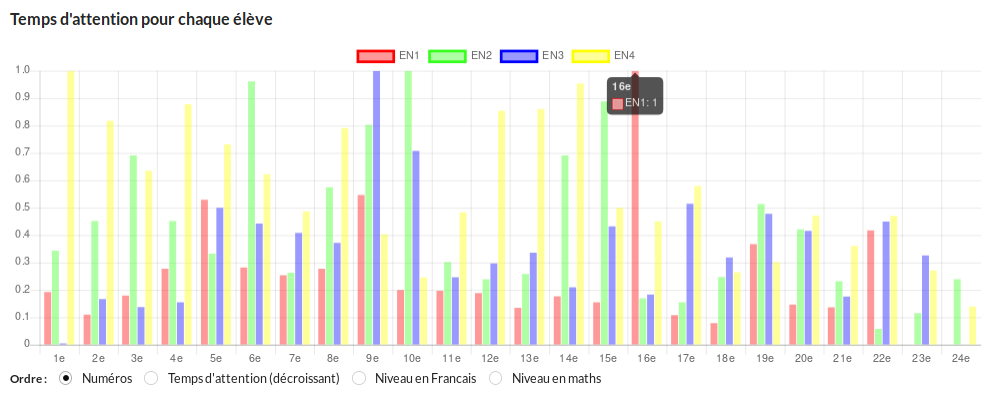
\includegraphics[height=4cm]{resume.png}
        \end{center}
        C'est cette page qui permet le mieux de visualiser la différence entre les enseignants (et en particulier entre les enseignants novices et les enseignants expérimentés).\\
    \item \textbf{Timelines:} Cette page reproduit les fonctionnalités du site \href{http://superviseur.lip6.fr/}{SuperViseur} original. On peut y voir les regards de l'enseignant en fonction du temps, soit par élève, soit groupé par niveau en français ou en mathématiques. On peut dans tous les cas bénéficier de plus d'informations sur un élève en passant le curseur au dessus des parties de la timelines lui correspondant. 
        \begin{center}
            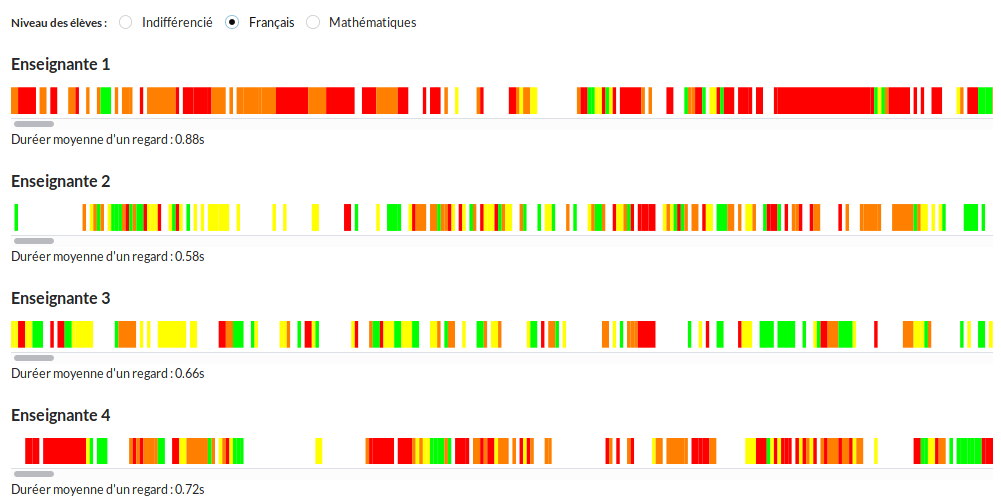
\includegraphics[height=5cm]{timelines.png}
        \end{center}
        Il est a noter que cette page prends malheureusement un peu de temps à charger, à cause principalement du grand nombre de rectangles à dessiner pour représenter les timelines.\\
    \item \textbf{Représentation circulaire:} Cette représentation est la première s'intéressant à la position spatiale des étudiants et de l'enseignant lors de la séance. Une fois l'option "Position de l'enseignant" activée, la distance entre les points représentant les élèves et le centre (représentant l'enseignant) correspond à la distance dans la salle de classe (quand les vrais données seront en place en tout cas, puisque comme mentionné plus haut, on utilise pour le moment des données factices pour la position).
        \begin{center}
            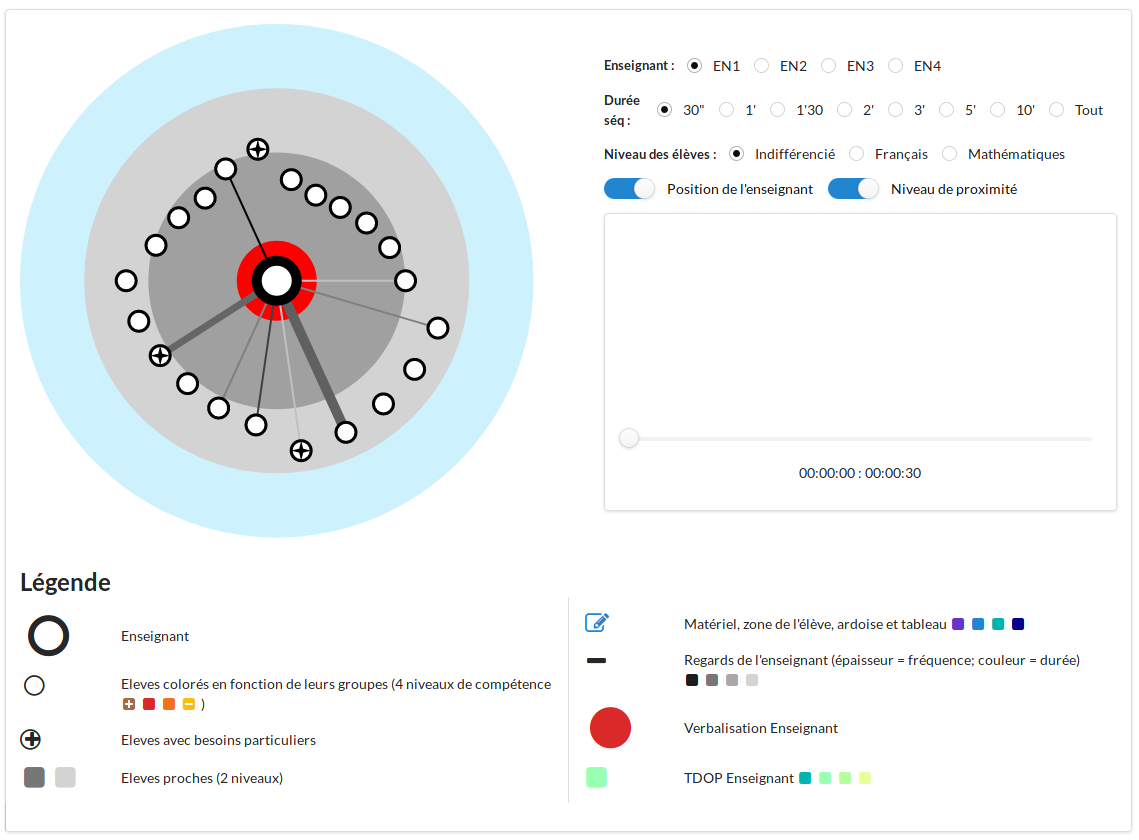
\includegraphics[height=7cm]{rep_circulaire.png}
        \end{center}
        Une fois de plus, les étudiants peuvent être triés par niveau en français ou en mathématiques (ce qui se matérialise par la couleur des cercles les représentants). On peut se déplacer temporellement dans la période du cours en utilisant un slider, et avec différents intervalles de temps, allant de 30 secondes à 10 minutes. On peut également afficher un résumé pour l'intégralité de la séance.\\
    \item \textbf{Représentation spatiale:} Plus encore que la représentation circulaire, la représentation spatiale s'intéresse au déplacement de l'enseignant dans la classe. Cette visualisation rends compte de la position des élèves grace aux données de position contenues dans le fichier \textit{users.csv}. Une fois l'option "Position de l'enseignant activée" on peut aussi suivre le déplacement de l'enseignant (on utilise pour le moment les données factices).
        \begin{center}
            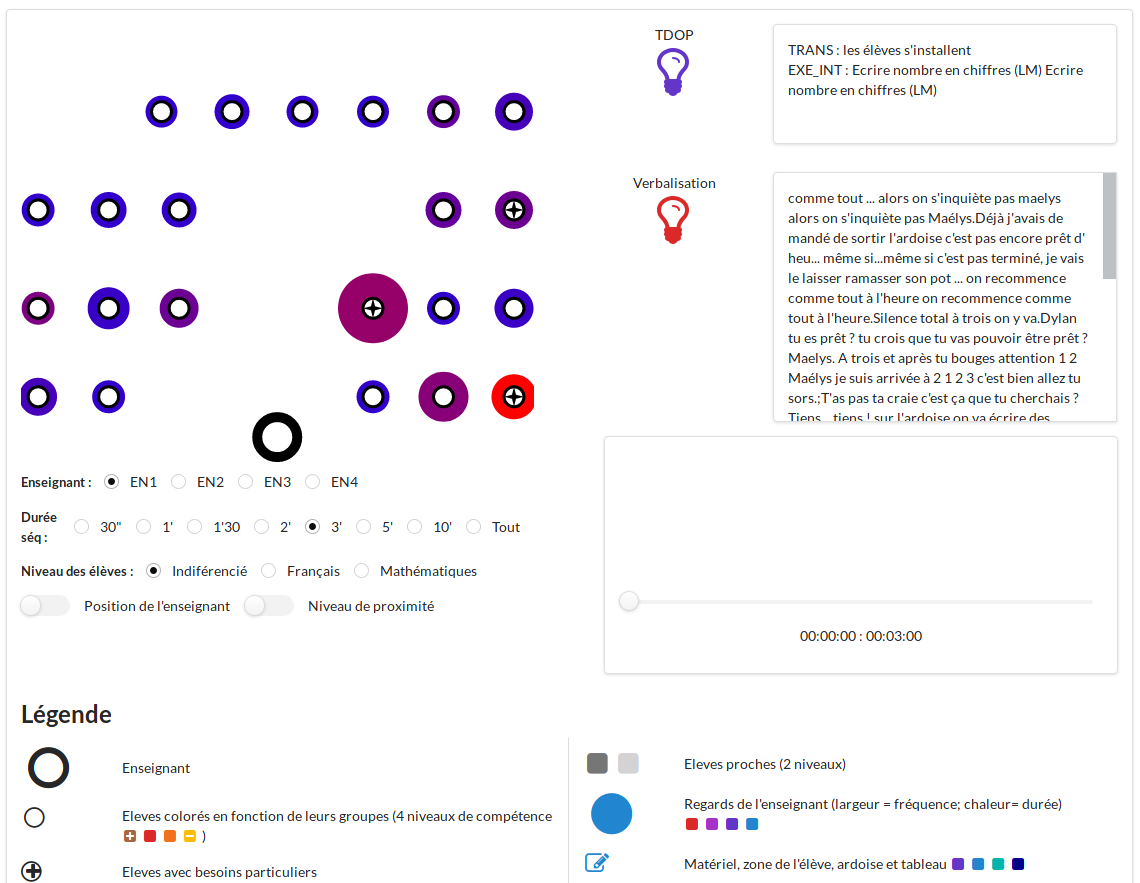
\includegraphics[height=7cm]{rep_spatiale.png}
        \end{center}
        En plus des informations affichées sur la visualisation précédente, on affiche aussi sur cette page la verbalisation de l'enseignant, ainsi que le(s) TDOP~\cite{TDOP} durant la période visualisée (code et description de l'action).
\end{itemize}

\section{Tests utilisateurs}
Afin de valider l'ergonomie du site réalisé, on a organisé une séance de tests utilisateurs.

\subsection{Protocole de test}
Lors du test, les utilisateurs ont eu à accomplir une série de taches en utilisant le site SuperViseur. Comme ce site présente principalement des visualisations, ces taches consistaient principalement à trouver des informations en ce servant des différentes visualisations présentes sur le site.
\begin{itemize}
    \item Quel est le premier élève que regarde l'enseignant 4 durant le cours?
    \item Qui sont les enseignants novices et qui sont les enseignants experts?
    \item Quel est l'enseignant qui distribue le plus son attention (coefficient GINI le moins élevé)?
    \item Combien y'a t-il d'élèves ayant des besoins particuliers dans la classe de l'enseignant 1?
    \item Quel est l'élève le plus regardé par l'enseignant 3? 
    \item Quels catégories d'enseignants (novices ou experts) regardent le plus les élèves ayant des difficultés en Francais (niveau faible ou passable)?
    \item L'enseignant 2 regarde-t-il plus souvent les élèves ayant un niveau en maths passable ou très bon?
    \item Quelle était le TDOP à l'ouverture du cours de l'enseignant 1?
    \item Quel est l'enseignant qui a les regards les plus longs?
\end{itemize}

\subsection{Résultats}

\section{Observations}
On rappelle que les enseignants les plus expérimentés sont les enseignants 1 et 4 (plus de 20 ans d'expérience) tandis que les enseignants 2 et 3 ont tous les deux moins d'une année d'expérience. Comme on va le voir, les différences entre les enseignants novices et expérimentés sont, comme on en avait fait l'hypothèse, nombreux.
\subsection{Représentations spatiales}
D'un point de vue des représentations spatiales, on s'aperçoir que les enseignants regardent plus fréquemment les élèves situés aux premiers rangs de la classe. On observe d'ailleurs que la disposition des élèves dans la salle ne semble pas dépendre de leur niveau, et n'est donc pas la raison des différences d'attention entre les niveaux. L'enseignant 4 (qui est expérimenté) est cependant une exception a ce principe, puisuq'il semble placer les élèves les plus en difficultés aux premiers rangs et ceux ayant le meilleur niveau au fond de la salle.\\
Malheureusement, comme on l'a vu plus haut, on ne possède pas les données nécessaires pour étudier le déplacement de l'enseignant dans la classe.

\subsection{Différences entre novices et expérimentés}
On remarque que l'attention des enseignants débutants est plus "fragmentée": en effet la durée moyenne de leurs regards est plus courte (0.58 et 0.66s, contre 0.72 et 0.88s pour les enseignants expérimentés). Cela peut être interprété comme une plus grande difficulté à évaluer l'état de la classe, et donc à une plus grande charge cognitive.\\
Tous les enseignants apportent plus d'attention aux élèves de niveau "Faible" ou "Passable", mais cette tendance est plus marquée chez les enseignants les plus expérimentés.
Les coefficients GINI en revanche ne permettent pas de différencier les enseignants novices et experimentés: tous les coefficients sont situés entre 0.24 et 0.35. L'enseignant ayant le coefficient le plus faible (0.24), et donc qui partage son attention de la façon la plus équitable est expérimenté (l'enseignant 4), mais l'enseignant 1 qui est lui aussi expérimenté a le coefficient le plus fort (0.349).\\

\subsection{Groupes de référence}
On constate que les groupes de références sont de taille assez variable. Pour les enseignants 1 et 3, ils ne comptent qu'un seul élève (respectivement l'élève 16 et l'élève 9) qui est considérablement plus regardé que l'élève en deuxième position. L'enseignant 2 lui consacre la plus grande partie de son attention sur les élèves 10, 6 et 15. Enfin, l'enseignant 4 (qui comme on l'a vu à un coefficient GINI très élevé regarde majoritairement les élèves 1, 14, 4, 13 et 12).\\
La taille du groupe de référence ne semble donc pas dépendre du niveau d'expérience de l'enseignant. On observe aussi que les élèves faisant partie des groupes de références sont tous en difficulté ne mathématiques (niveau "Faible" ou "Passable") ou ont des besoins particuliers. Cela est bien sur en adéquation avec nos observations précédentes.
\begin{center}
    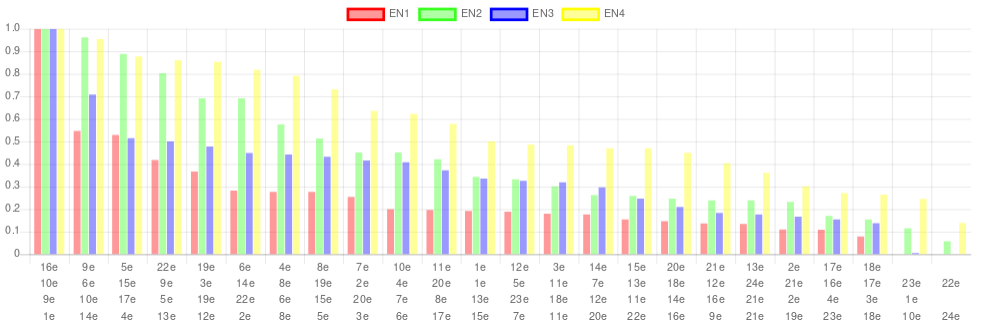
\includegraphics[height=4cm]{ordre_decroissant.png}
\end{center}

\section{Conclusion}

\bibliography{bibliographie}{}
\bibliographystyle{plain}
\end{document}
